\section {Assignment 2 \\ {Object in front of Dark Background}}
\label {sec:assignment_2}

For this assignment, we will be capturing a image wich we will also use for assignment 3 and 4. It will be of a model car in front of a dark background. 
The goal is to make a useful setup to acquire the image and solely adjust the exposuretime to come to a well exposed image \cite{Lab_Assignments}.

The code in Listing \ref{lst:expose_time_image} was used to take the image, or adjust the exposure time. The image was then saved in the folder from wich the program was run. for the full code see appendix \ref{sec:appendix_A}.

\begin{lstlisting}[language=C, caption=save image to file, label=lst:expose_time_image]
    case ' ':
        if (imgSave(image, "output.png")) {
            cout << "Image saved succesfully!" << endl;
        } else {
            cout << "Error saving file." << endl;
        }
        break;
        case ',':
        cam0.setExpoMs(--cfg.exposureMS);
        cout << "Exposure adjusted to " << cfg.exposureMS << endl;
        break;
        case '.':
        cam0.setExpoMs(++cfg.exposureMS);
        cout << "Exposure adjusted to " << cfg.exposureMS << endl;
        break;
        case '[':
        cam0.setExpoMs(cfg.exposureMS -= 10);
        cout << "Exposure adjusted to " << cfg.exposureMS << endl;
        break;
        case ']':
        cam0.setExpoMs(cfg.exposureMS += 10);
        cout << "Exposure adjusted to " << cfg.exposureMS << endl;
        break;
\end{lstlisting}

\subsection{Object with dark background}

\begin{figure}[h!]
    \centering
    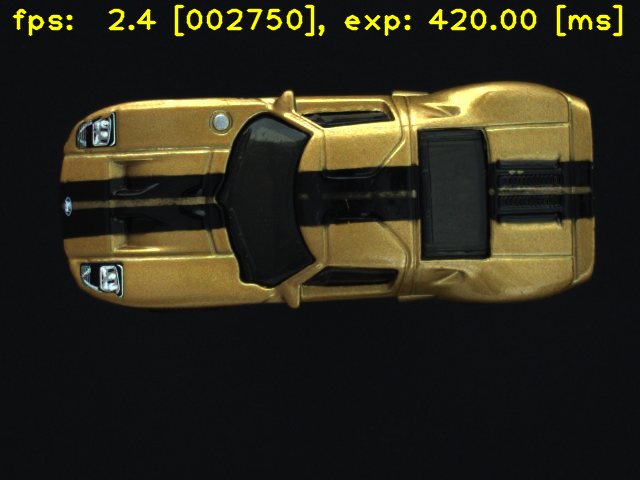
\includegraphics[width=0.45\textwidth]{ford_gt_final2.png}
    \caption{Object in front of Dark Background}
    \label{fig:fortgt}
\end{figure}

The image above is the image we took of the model car, it has a matelic gold paint with black stripes across. It was challenging to get the car well exposed, because the metallic paint is reflective. So we needed even light positioned in a way that the reflections would not go into the camera. Enough light was needed for the black parts of the car to not be ender exposed. We placed the object away from the background so we could make shine the light only on the car and not the background. The layout of the setup is shown in section \ref{sec:sketch}.

\subsection{Optimal exposure}

We got the best result using a 420 ms exposure time. This is the time the camera takes to gather light on the sensor. The image is shown in figure \ref{fig:fortgt}. The image is well exposed and the background is dark. The car is well visible and the details are clear. The image is not overexposed and the background is black but not saturated. 

\subsection{Sketch of setup}
\label{sec:sketch}

\begin{figure}[H]
    \centering
    \includegraphics[width=0.5\textwidth]{Lab_2_Diagram.png}
    \caption{Sketch of setup}
    \label{fig:sketch}
\end{figure}

\subsection{Calculation of ‘angle of view’}
\label{sec:angle_of_view}

% \begin{figure}[h!]
%     \centering
%     \includegraphics[width=0.35\textwidth]{ford_gt_final2_dimensies.png}
%     \caption{Angle of view reference image}
%     \label{fig:angleofview}
% \end{figure}

% The (horisontal) angle of view is the angle between the left and right part of the frame, and the camera lens. In order to calculate this we took a picture of a measuring tape stretching the full width of the frame at a known distance, 250 mm. See figure \ref{fig:angleofview} for this image. Now we calculate the angle of view:

% $$ \text{framewidth} = 90\text{mm} $$
% $$ \text{distance} = 250\text{mm}$$

% \begin{equation}
%     \theta = 2 \cdot \arctan{\frac{{\frac{\text{framewidth}}{2}}}{\text{distance}}} = 2 \cdot \arctan{\frac{\frac{90}{2}}{250}} = 2 \cdot \arctan{\frac{45}{250}} = 2 \cdot 19.8 = 39.6 \text{ degrees}
% \end{equation}

To calculate the angle of view $ \alpha $ we need the following information:

\begin{itemize}
    \item Sensor size [mm] $ d = 8.89 mm $
    \item focal length $ f = 6 mm $
\end{itemize}

And we used the following formula:

$$ \alpha = \frac{180}{\pi} \cdot 2\arctan{\frac{d}{2 \cdot f}} = \frac{180}{\pi} \cdot 2\arctan{\frac{8.89}{2 \cdot 6}} = 73.1 \text{ degrees} $$
